%%%%%%%%%%%%%%%%%%%%%%%%%%%%%%%%%%%%%%%
% a0poster Landscape Poster
% LaTeX Template
% Version 1.0 (22/06/13)
%
% The a0poster class was created by:
% Gerlinde Kettl and Matthias Weiser (tex@kettl.de)
% 
% This template has been downloaded from:
% http://www.LaTeXTemplates.com
%
% License:
% CC BY-NC-SA 3.0 (http://creativecommons.org/licenses/by-nc-sa/3.0/)
%
%%%%%%%%%%%%%%%%%%%%%%%%%%%%%%%%%%%%%%%%%

%----------------------------------------------------------------------------------------
%	PACKAGES AND OTHER DOCUMENT CONFIGURATIONS
%----------------------------------------------------------------------------------------

% maize2018 is 33'' x 46'' (84cm x 118cm)
\documentclass[maize,portrait]{a0poster}

\usepackage{fontspec}
\usepackage[svgnames]{xcolor} % enable specifying colors by their 'svgnames', for a full list of all colors available see here: http://www.latextemplates.com/svgnames-colors

% Carnegie uses Roboto Slab (serif) and Lato (sans serif)
\setmainfont[Ligatures=TeX]{Lato}

% Carnegie colors
\definecolor{CarnegiePriBlue}{cmyk}{1.00,0.85,0.15,0.25}  % main primary blue
\definecolor{CarnegieSecBlue1}{cmyk}{0.68,0.48,0.00,0.00} % first secondary blue
\definecolor{CarnegieSecBlue2}{cmyk}{0.85,0.69,0.04,0.00} % second secondary blue

\definecolor{CarnegiePriTurq}{cmyk}{0.60,0.10,0.15,0.00}  % main primary turquoise

\definecolor{CarnegiePriGreen}{cmyk}{0.46,0.00,0.90,0.00} % main primary green

\definecolor{CarnegiePriBrown}{cmyk}{0.25,0.40,0.65,0.00} % main primary brown

% multiple columns
\usepackage{multicol} % This is so we can have multiple columns of text side-by-side
\columnsep=100pt      % This is the amount of white space between the columns in the poster
\columnseprule=3pt    % This is the thickness of the black line between the columns in the poster
\def\columnseprulecolor{\color{lightgray}}

% other needed packages
\usepackage{amsfonts, amsmath, amsthm, amssymb} % For math fonts, symbols and environments
\usepackage{wrapfig}  % Allows wrapping text around tables and figures
\usepackage{graphicx} % Required for including images
\usepackage{booktabs} % Top and bottom rules for table

% tweak figure and table captions
\usepackage[font=small,labelfont={bf,color=CarnegiePriBlue},textfont={color=CarnegiePriBlue},margin=0pt,skip=18pt]{caption}

% natbib drops numbers and we'll shrink text size; drop labels
\usepackage{natbib}
\def\bibfont{\footnotesize}
\makeatletter
\renewcommand\@biblabel[1]{}
\makeatother

% tweak list spacing
\usepackage{enumitem}
\setlist[itemize]{topsep=10pt,itemsep=8pt,itemindent=48pt}
\setlist[enumerate]{topsep=10pt,itemsep=8pt,itemindent=0pt}


% tweak paragraphs
\setlength{\parindent}{0pt}
\setlength{\parskip}{12pt}

% tweak title spacing and colors
% \titlespacing{command}{left spacing}{before spacing}{after spacing}[right]
% spacing: how to read {12pt plus 4pt minus 2pt}
%          12pt is what we would like the spacing to be
%          plus 4pt means that TeX can stretch it by at most 4pt
%          minus 2pt means that TeX can shrink it by at most 2pt
\usepackage{titlesec}

\titlespacing{\section}{0pt}{24pt}{12pt}
\titlespacing{\subsection}{0pt}{12pt}{12pt}
\titlespacing{\subsubsection}{0pt}{12pt}{12pt}

\titleformat{\section}{\color{CarnegiePriBlue}\Large\bfseries}{\color{CarnegiePriBlue}\thesection}{1em}{}
\titleformat{\subsection}{\color{CarnegiePriBrown}\large\bfseries}{\color{CarnegiePriBrown}\thesubsection}{1em}{}

% tweak equation whitespace
%% \abovedisplayskip=12pt plus 3pt minus 9pt
%% \abovedisplayshortskip=0pt plus 3pt
%% \belowdisplayskip=12pt plus 3pt minus 9pt
%% \belowdisplayshortskip=7pt plus 3pt minus 4pt

% width of figures for consistency
\newlength{\figwidth}
\setlength{\figwidth}{240mm}

% space above figures
\newlength{\figtopspace}
\setlength{\figtopspace}{10pt}

\graphicspath{{figures/}} % Location of the graphics files

%% % DEBUG: overlay a grid to view spacing
%\usepackage[grid,gridcolor=red!20,subgridcolor=green!20,gridunit=in]{eso-pic}

\begin{document}

%----------------------------------------------------------------------------------------
%	POSTER HEADER 
%----------------------------------------------------------------------------------------

% The header is divided into three boxes:
% The first is 55% wide and houses the title, subtitle, names and university/organization
% The second is 25% wide and houses contact information
% The third is 19% wide and houses a logo for your university/organization or a photo of you
% The widths of these boxes can be easily edited to accommodate your content as you see fit
% Note: no line breaks between minipage environments!

\textbf{\color{CarnegiePriBlue} \VeryHuge GBS identification of genomic loci associated with embryo twins in \textit{ig1} mutants}    % Title

\begin{minipage}[m]{0.08\linewidth}
  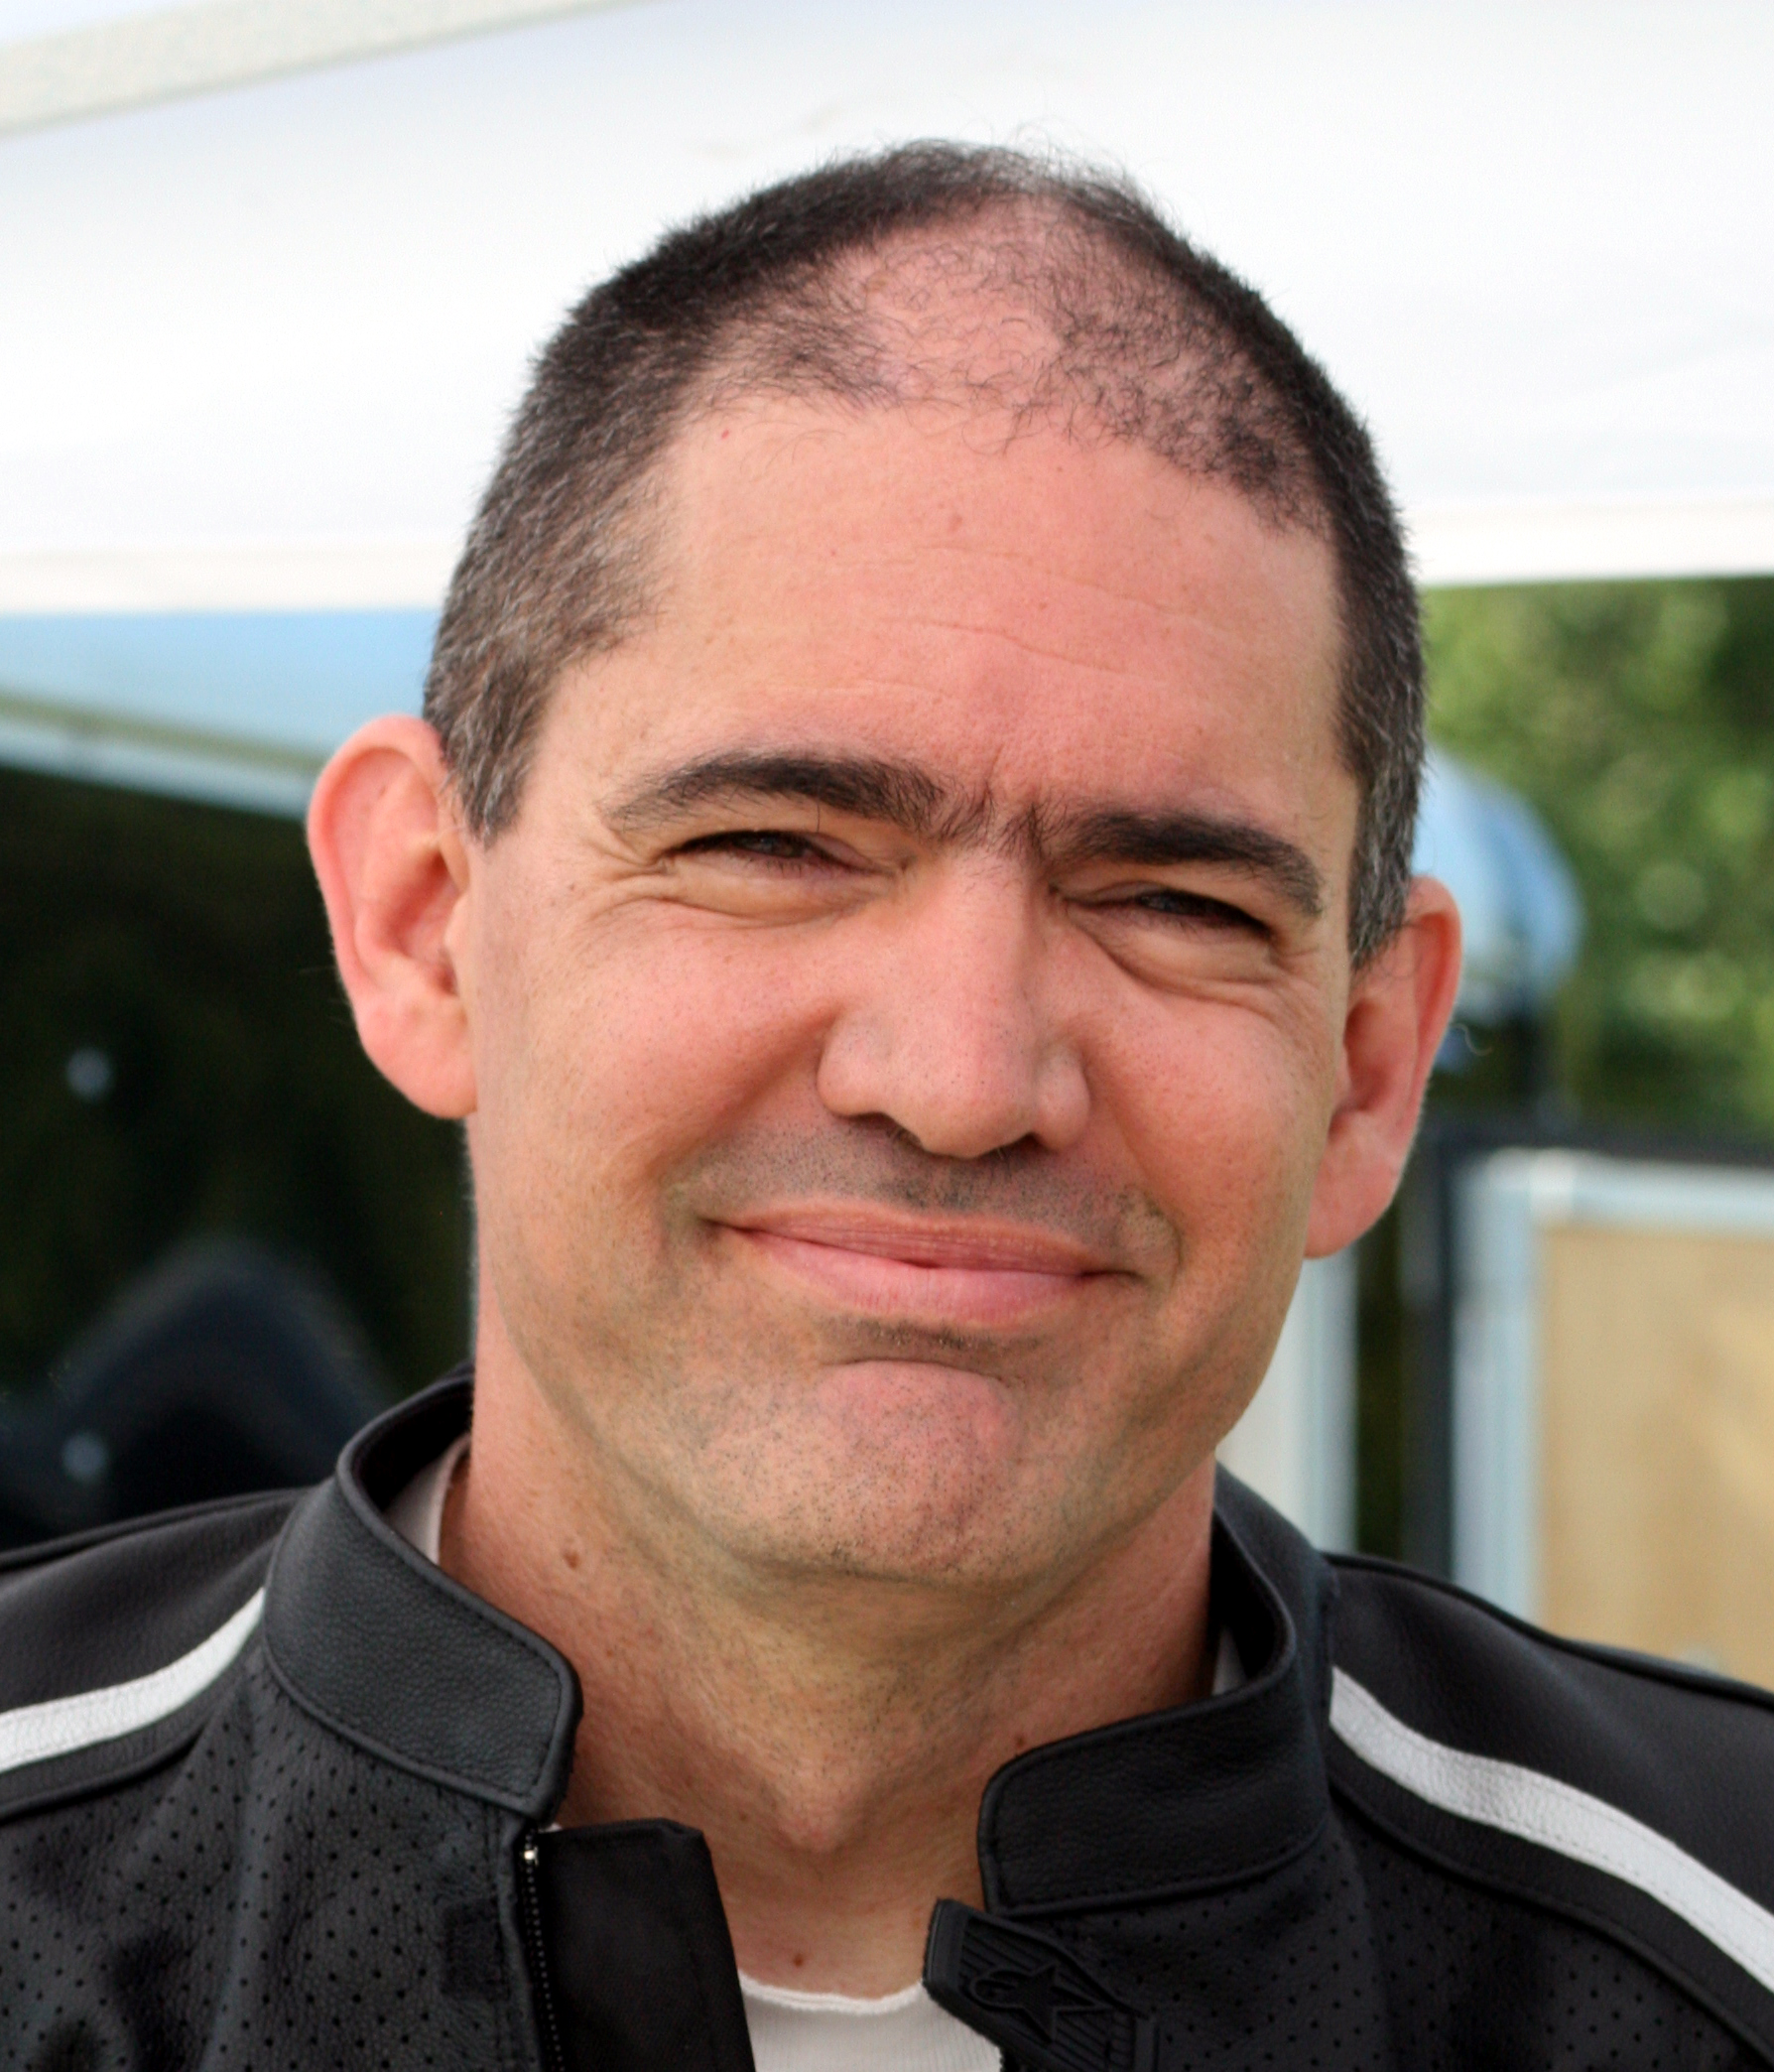
\includegraphics[height=50mm]{sam-bfr-smiling-crop.jpg} % author photo
\end{minipage}
\begin{minipage}[m]{0.50\linewidth}                      % Author(s)
  \color{Black}
  \Huge \textbf{Sam Hokin, Matt Evans, Antony Chettoor \& Vicki Tang} \\
  \Large shokin@carnegiescience.edu
\end{minipage}
\hfill
\begin{minipage}[m]{0.40\linewidth}                      % Author(s)
  \hfill
  
\includegraphics[height=50mm]{CS_plantbio_logo_horz.eps} % Carnegie DPB logo
\end{minipage}

\vspace{5mm} % A bit of extra whitespace between the header and poster content
\color{CarnegiePriBlue}
\hrulefill

\color{Black}

%% \color{DarkSlateGray}\Large \textbf{Contact Information:}\\
%% Department Name\\ % Address
%% University Name\\
%% 123 Broadway, State, Country\\\\
%% Phone: +1 (000) 111 1111\\ % Phone number
%% Email: \texttt{john@LaTeXTemplates.com}\\ % Email address


%----------------------------------------------------------------------------------------

\begin{multicols}{4} % This is how many columns your poster will be broken into, a poster with many figures may benefit from less columns whereas a text-heavy poster benefits from more

  \color{Black} % default color

  %----------------------------------------------------------------------------------------
  %	ABSTRACT
  %----------------------------------------------------------------------------------------

  %% \begin{abstract}
  %% \end{abstract}

  %----------------------------------------------------------------------------------------
  %	INTRODUCTION
  %----------------------------------------------------------------------------------------

  {
    \titlespacing{\section}{0pt}{0pt}{0pt} % suppress skip on very first section
    \section*{INTRODUCTION}
  }

  \textbf{Stuff.}

  More stuff.
  
  %----------------------------------------------------------------------------------------
  %	OBJECTIVES
  %----------------------------------------------------------------------------------------

  \section*{OBJECTIVES}
  \color{CarnegiePriBlue}  

  \begin{enumerate}
  \item Stuff 1
  \item Stuff 2
  \item Stuff 3
  \item Stuff 4
  \end{enumerate}

  \color{Black}

  %----------------------------------------------------------------------------------------
  %	MATERIALS AND METHODS
  %----------------------------------------------------------------------------------------

  \section*{MATERIALS AND METHODS}

  %% Could have introductory text here before subsections.

  %------------------------------------------------

  \subsection*{Subsection}

  Stuff.

  \subsection*{Another subsection}

  More stuff.

  %----------------------------------------------------------------------------------------
  %	RESULTS 
  %----------------------------------------------------------------------------------------

  \section*{RESULTS}

  \subsection*{Subsection}

  Stuff.

  \subsection*{Another subsection}

  More stuff.
  
  %----------------------------------------------------------------------------------------
  %	CONCLUSIONS
  %----------------------------------------------------------------------------------------

  \section*{CONCLUSIONS}
  \color{CarnegiePriBlue}
  
  \begin{enumerate}
  \item Conclusion 1
  \item Conclusion 2
  \item Conclusion 3
  \end{enumerate}

  %----------------------------------------------------------------------------------------
  %	FURTHER RESEARCH
  %----------------------------------------------------------------------------------------

  \section*{Further Research}
  
  \begin{enumerate}
  \item Do this 1
  \item Do this 2
  \item Do this 3
  \item Do this 4
  \end{enumerate}

  %----------------------------------------------------------------------------------------
  %	REFERENCES
  %----------------------------------------------------------------------------------------

  \nocite{*} % Print all references regardless of whether they were cited in the poster or not
  \bibliographystyle{plain} % Plain referencing style
  \bibliography{hokin-maize2018} % Use hokin-maize2018.bbl - regenerate with bibtex

  %----------------------------------------------------------------------------------------
  %	ACKNOWLEDGEMENTS
  %----------------------------------------------------------------------------------------

  {\small This research was funded by National Science Foundation grant \#XXXXXXX.}
  
  
\end{multicols}
\end{document}
